% This work is licensed under the Creative Commons Attribution-NonCommercial 4.0 International License.
% To view a copy of this license, visit http://creativecommons.org/licenses/by-nc/4.0/
% or send a letter to Creative Commons, PO Box 1866, Mountain View, CA 94042, USA.

% !TEX TS-program = xelatex

\documentclass[../Main/chem371-notes.tex]{subfiles}

\setcounter{chapter}{0}
\begin{document}

\chapter{The Basics of Quantum Chemistry}

(updated \today)

\section{What is Quantum Chemistry?}
According to Wikipedia:
\begin{quotation}
Quantum chemistry, also called molecular quantum mechanics, is a branch of chemistry focused on the application of quantum mechanics in physical models and experiments of chemical systems. Understanding electronic structure and molecular dynamics using the Schrödinger equations are central topics in quantum chemistry.
\end{quotation}

Quantum chemistry, and more generally, computational chemistry is a growing subfield of chemistry.
Its main purpose is to use quantum physics to predict the physical and chemical properties of molecules and materials, understand the mechanism of reactions, and connect experimental measurements (e.g., from spectroscopy) to molecular structure.
The potential revolutionary impact that quantum mechanics may have on chemistry was recognized in the early days of quantum mechanics by Paul Dirac, who wrote:\mnote{Proceedings of the Royal Society of London. Series A, Containing Papers of a Mathematical and Physical Character, Vol. 123, No. 792 (6 April 1929)}
\begin{quotation}
The underlying physical laws necessary for the mathematical theory of a large part of physics and the whole of chemistry are thus completely known, and the difficulty is only that the exact application of these laws leads to equations much too complicated to be soluble.
It therefore becomes desirable that approximate practical methods of applying quantum mechanics should be developed, which can lead to an explanation of the main features of complex atomic systems without too much computation.
\end{quotation}

Here we encounter one common theme of this course: that due to the difficulties of applying quantum mechanics to chemistry, we will only have access to approximate solutions.
This implies that we will have methods that introduce errors, and we will have to develop an understanding what limitations each method has.

\section{Quantum Mechanics and the Schr\"{o}dinger equation}
The basic equation at the basis of quantum mechanics is the Schr\"{o}dinger equation\mnote{This is the \emph{time-independent} version of the Schr\"{o}dinger equation. The more general version is the time-dependent form, which can be applied to study dynamical process.}
\begin{iequation}
\hat{H}\Psi = E \Psi
\end{iequation}
\mdef{Hamiltonian}{the quantum mechanical operator $\hat{H}$.}
\mdef{Wave function}{$\Psi$ / $\psi$ (pronounced ``psahy''). Represents the state of a quantum system.}
This equation contains three elements:
\begin{myitems}
\item The \emph{Hamiltonian operator} $\hat{H}$. This is a mathematical operator, in the sense that when it is applied to a function it produces a new one. The Hamiltonian contains terms for the kinetic and potential energy.
\item The \emph{wave function} $\Psi$. This is a function of the coordinates of all the particle in a quantum system and contains all the information necessary to describe the state of a quantum system.
\item The \emph{energy} $E$. This is the energy (a real number) that corresponds to the wave function $\Psi$.
\end{myitems}
The Schr\"{o}dinger is an \emph{eigenvalue} equation, because it says that when we apply the Hamiltonian to the wave function we get back the wave function times a number (the energy).

For a molecule, the wave function depends on the coordinates of the electrons and nuclei.
For example, for one electron the wave function is a function of the electron position vector $\mathbf{r} = (x,y,z)$ specified by the the Cartesian coordinates $x,y,z$, $\Psi(\mathbf{r})$.
From quantum mechanics, we know that the wave function should be interpreted as a \emph{probability amplitude}, that is, if we take the modulus square the wave function we get the probability that the electron is in position $\mathbf{r}$
\begin{equation}
P(\mathbf{r}) \equiv \text{ probability of finding the electron in position } \mathbf{r} = |\Psi(\mathbf{r})|^2  = \Psi^*(\mathbf{r}) \Psi(\mathbf{r}) 
\end{equation}
For this probabilistic interpretation to make sense, the sum of the probability of finding the electron in the whole space must add to one, that is, the wave function should satisfy the \emph{normalization} condition
\begin{equation}
\int  d\mathbf{r} \; P(\mathbf{r}) =  \int _{-\infty}^{\infty} dx \int _{-\infty}^{\infty} dy \int _{-\infty}^{\infty} dz \; |\Psi(\mathbf{r})|^2   = 1
\end{equation}
This equation says that if we integrate (sum) the probability of finding one electron over all space, it must add up to one.

Once we have an exact or approximate wave function we can compute the \emph{expectation value} (average value) of an operator corresponding to a quantity that we might want to determine.
For example, to find out the energy we compute the expectation value of the Hamiltonian
\begin{equation}
E = \int \Psi^* \hat{H} \Psi
\end{equation}
where the integral runs over all positions of the particle in our system.\mnote{This result generalizes to any operator. If the operator $\hat{O}$ corresponds to the observable $O$, then the expectation value  of $O$ is given by
\begin{equation}
\braket{O}= \int \Psi^* \hat{O} \Psi
\end{equation}
}

As pointed out by Dirac, the Schr\"{o}dinger equation is hard to solve!
There are only very few systems for which one can find exact solutions of the Schr\"{o}dinger equation.
These include a particle in a box, the harmonic oscillator, a rotating molecule.
The next example discusses the particle in a box.

\begin{example}[The particle in a box]
\mfigure{
\centering{
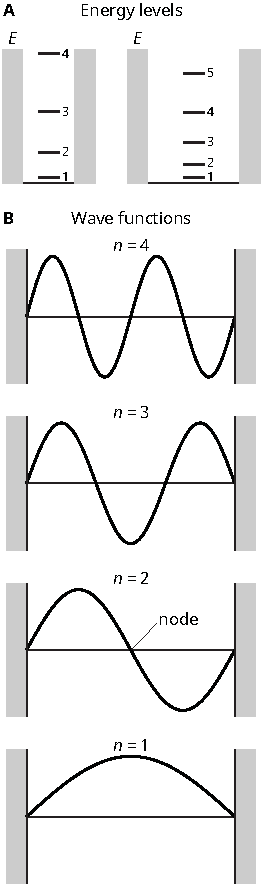
\includegraphics[width=1.75in]{img/pib.pdf}
}
\captionof{figure}{Particle trapped in a one-dimensional box. (\textbf{A}) the first few energy levels as a function of the quantum number $n = 1, 2, \ldots$ for a narrow (left) and wide (right) box. (\textbf{B}) The first four wave functions of the particle in a box.}
\label{fig:pib}
}

In this example we examine one of the simplest problems in quantum mechanics that can be solved exactly: a particle trapped in a one-dimensional box.
We assume that the box has length $L$, and it runs from 0 to $L$.
For this toy model the Hamiltonian is given by
\begin{equation}
\hat{H} = -\frac{\hbar^2}{2m} \frac{d^2}{dx^2}.
\end{equation}
The Schr\"{o}dinger equation is given by
\begin{equation}
-\frac{\hbar^2}{2m} \frac{d^2}{dx^2} \psi(x) = E \psi(x).
\end{equation}
The solutions of this equation depend on a \emph{quantum number} $n = 1, 2, 3, \ldots$, an integer that goes from one to infinity.
The energy of the $n$th level is
\begin{iequation}
E_n = \frac{\hbar^2 n^2 \pi^2}{2m L^2} = \frac{h^2 n^2 }{8 m L^2}, \quad n = 1,2,3\ldots
\end{iequation}
while the corresponding wave functions are given by
\begin{iequation}
\psi_{n}(x) = \sqrt{\frac{2}{L}} \sin\left(\frac{n \pi x}{L}\right).
\end{iequation}
The energy levels and wave functions for the particle in a box are shown in Fig.~\ref{fig:pib}.
Here we see two important features of the Schr\"{o}dinger equation.
Firstly, the energy levels are discrete, a phenomenon that is referred to as quantization.
Since the energy is proportional to $1/L^2$, when we make the box wider, the spacing between the energy levels becomes smaller.
Note also that the lowest energy level ($n=1$) always has a positive energy, this is usually called the \emph{zero point energy}.

Secondly, the higher energy wave functions contain more nodes.
Here by a node we mean a point where the wave function is equal to zero.
This is a consequence of the fact that wave functions are orthogonal with respect to each other.
You have already encountered this phenomenon when you studied the atomic orbitals of the hydrogen atom.
For example, the 1s orbital has no nodes. The 2p orbitals (2p$_x$,2p$_y$,2p$_z$) have one nodal plane, etc.
\end{example}



\section{The Quantum Mechanics of Molecules}

In an atom or a molecule, where we have more than one particle, the wave function is a function of the coordinates of all the electrons ($\mathbf{r}_i$) and nuclei ($\mathbf{R}_i$)
\begin{equation}
\Psi(\mathbf{r}_1, \mathbf{r}_2, \ldots, \mathbf{R}_1,  \mathbf{R}_2,\ldots)
\end{equation}
The wave function must also satisfy another important property: it must be antisymmetric with respect to the interchange of electrons. We will return to this point later.

The Hamiltonian operator depends on the coordinates ($\mathbf{r}_i$) and the charges ($q_i$) of all the particles, and it can be separated into a kinetic energy operator plus a potential operator
\begin{align}
\hat{H} & =
\underbrace{
\sum_i -\frac{1}{2 m_i} \nabla^2_i
}_{\text{kinetic}}
+
\underbrace{
\frac{1}{4\pi \epsilon_0} \sum_{i < j} \frac{q_i q_j}{r_{ij}}
}_{\text{potential (Coulomb)}}  
\\
\nabla^2_i & = \frac{\partial^2}{\partial x_i^2} +  \frac{\partial^2}{\partial y_i^2} +  \frac{\partial^2}{\partial z_i^2}
\end{align}
where $r_{ij} = |\mathbf{r}_i - \mathbf{r}_j|$ is the distance between particles $i$ and $j$ and the symbol $\nabla^2_i$ is the Laplacian operator acting on particle $i$.
Since the electron and nuclei interact via their electric charge, the potential is just the classical Coulomb potential.

\mfigure{
\centering{
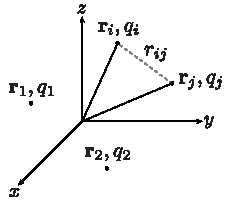
\includegraphics[width=1.75in]{img/molecule.pdf}
}
\captionof{figure}{In quantum mechanics, a molecule is a collection of particles with position vector $\mathbf{r}_i$ and charge $q_i$. The distance between particles $i$ and $j$ is $r_{ij} = |\mathbf{r}_i - \mathbf{r}_j|$.}
}

In a molecule, where we have electrons and nuclei, we can separate terms that refer to electron (e) and nuclear (n) coordinates
\begin{equation}
\hat{H} = \hat{T}_\mathrm{e} + \hat{T}_\mathrm{n} +  \hat{V}_\mathrm{ee} + \hat{V}_\mathrm{en} + \hat{V}_\mathrm{nn}
\end{equation}
In this equation $\hat{T}_\mathrm{e}$ is the kinetic energy of the electrons
\begin{equation}
\hat{T}_\mathrm{e} = -\frac{1}{2 m_e}  \sum_{i}^{\mathrm{electrons}}\nabla^2_i
\end{equation}
$\hat{V}_\mathrm{ee}$ is the electron-electron potential energy ($q_i = q_j = - q_e$), which is always positive
\begin{equation}
\hat{V}_\mathrm{ee} = \frac{q_e^2}{4\pi \epsilon_0}  \sum_{i < j}^{\mathrm{electrons}} \frac{1}{|\mathbf{r}_{i} - \mathbf{r}_{j}|}
\end{equation}
and $\hat{V}_\mathrm{en}$ is the electron-nuclear potential energy (for electrons $q_i = -q_e < 0$, for nuclei $q_j > 0$), which is always negative
\begin{equation}
\hat{V}_\mathrm{en} = - \frac{q_e}{4\pi \epsilon_0}  \sum_{i}^{\mathrm{electrons}}  \sum_{j}^{\mathrm{nuclei}} \frac{q_j}{|\mathbf{r}_{i} - \mathbf{R}_{j}|}
\end{equation}
The other terms are defined in a similar way.

In principle, to predict the energy and properties of atoms we could solve the Schr\"{o}dinger equation for a molecule
\begin{equation}
\hat{H} \Psi(\mathbf{r}_1, \mathbf{r}_2, \ldots, \mathbf{R}_1,  \mathbf{R}_2,\ldots) = E \Psi(\mathbf{r}_1, \mathbf{r}_2, \ldots, \mathbf{R}_1,  \mathbf{R}_2,\ldots)
\end{equation}
However, in the next chapter we will see that there is an important approximation that we can make and that simplifies this problem a bit.

\section{Atomic units}
When doing computations on atoms or molecules it is convenient to use \emph{atomic units} (abbreviated a.u.), which are defined by the following conditions
\begin{align}
\text{electron mass} & = m_e = 1\\
\text{electron charge} & = e = 1\\
\text{action} & = \hbar = \frac{h}{2\pi} = 1\\
\text{Coulomb's constant} & = k_e = \frac{1}{4\pi \epsilon_0} = 1
\end{align}
These are natural units because the charge and mass of the particles we want to describe (electrons) are close to one.
In practice, it means that we will often avoid carrying around powers of ten in computations.

Another good reason for using atomic units is that computations done in the units involve numbers that are close to one, and because computers always use approximate representations for real numbers, the results will be less affected by roundoff errors.
All computer programs that perform quantum chemistry computations on molecules adopt atomic units.
So you will often have to convert results from atomic units to SI or other units that are commonly used in chemistry.

Two of the most useful atomic units are the \emph{hartree} (symbol  \Eh), the unit of energy, and the \emph{bohr}, the unit of length.
One hartree is a minuscule amount of energy, only about 4.36 $\times 10^{-18}$ Joules!
The energy changes that we measure in chemistry typically refer to one mole of matter, so a more convenient conversion factor is 
\begin{iequation}
1 \text{ hartee} = 627.51 \text{kcal/mol}
\end{iequation}
This factor converts energy differences for one atom/molecule to a mole of atoms/molecules.

\begin{example}[Strength of a carbon hydrogen bond in methane]
Breaking a \ce{C-H} bond in methane requires about 104 kcal/mol. When converted to hartree this quantity is 104/627.51 kcal/mol = 0.165 \Eh.
This is (approximately) the energy difference that you would get if you performed a quantum chemistry computation in which you compare the energy of one \ce{CH4} molecule with that of the \ce{CH3} radical plus one hydrogen atom.
\end{example}

\begin{example}[Chemical accuracy]
When modeling chemical reactivity, a common goal is to achieve an accuracy of 1 kcal/mol. When converted to atomic units this amount is equal to 1/627.51 \Eh = 0.0015936 \Eh.
\end{example}

One bohr is the most probable distance between the nucleus and the electron in a hydrogen atom, and when expressed in units of angstrom it is equal to
\begin{iequation}
1 \text{ bohr} = 0.52918 \text{ \AA{}}
\end{iequation}
Most computational chemistry programs \emph{assume} that the geometry of a molecule is specified using in units of \AA{}.
Alternatively, the user can specify that a molecular geometry is defined in units of bohr.
However, computations are typically done in units of bohr, and some times the output of a computation may be printed in these units.
It is always good to double check to avoid that a geometry is specified in the correct units.
A typical problem for beginners is confusing the two units.
In this case, it is easy to spot the problem because something strange typically happens is a computation (all the atoms in a molecule are far apart, or scrunched up).


The following table shows the name and conversion factors between atomic units and SI units:
\begin{table}[htbp]
\centering
\begin{tabular}{lll}
\toprule
Dimension & Symbol (Name) & Value in Other Units\\
\midrule
Length & $a_0$ (bohr) & 0.52918 \AA{}  = $0.52918 \times 10^{-10}$ m\\ 
Mass & $m_e$ & $9.1095 \times 10^{-31}$ Kg \\
Charge & $e$ & $1.6022 \times 10^{-19}$ C \\
Action & $\hbar$ & $1.05457 \times 10^{-34}$ J $\cdot$ s \\
%Coulomb's constant & $\frac{1}{4\pi \epsilon_0}$ & $ \times 10^{-34}$ J $\cdot$ s \\
Energy & $E_{\rm h}$ (hartree) & 627.51 kcal/mol \\
& & 27.211 eV \\
& & 219474.63 cm$^{-1}$ \\
& & $4.3598 \times 10^{-18}$ J\\
Time & & $2.41889 \times 10^{-17}$ s $\approx 1/41.3$ fs\\
\bottomrule
\end{tabular}
%\caption{Remember, \emph{never} use vertical lines in tables.}
\label{tab:atomicunits}
\end{table}

The speed of light in atomic units is $\alpha^{-1}\approx 137$ a.u.\mnote{The quantity $\alpha$ is also known as the fine-structure constant.}

\begin{aside}
\section*{Calculation or computation?}
What word should we use when we want to describe the result of some computational procedure used to determine the properties of molecule?
Often the words \emph{computation} and \emph{calculation} are used interchangeably, however, the word computation best conveys the meaning of the results of a mathematical calculation done with a computer. Here are dictionary definitions of these two terms:
\begin{quote}
Calculation: A mathematical determination of the size or number of something
\end{quote}
\begin{quote}
Computation: The action of mathematical calculation. The use of computers, especially as a subject of research or study.
\end{quote}
\end{aside}



\end{document}